\section{Introduction to Micro-service Architectures}
\label{sec:techKnowHow}
This section aims to elaborate the nature of microservices in a quite general matter. Therefore the term will be defined and distinguished between service-oriented-architectures (SOA) first of all. After having understood that crucial part the theory and benefits of self-contained-systems are introduced. This chapter will be finished by having a look upon event-based micro-service collaboration. Their advantages as well as disadvantages will be shown within that section. 

\subsection{Distinction between SOA and Microservice-Architectures}
Microservice Architecture is a quite commonly used buzz-word for a state of the art way of how to implement software. Having a look into the data of Google Trends it is possible to see that the popularity of this approach increases dramatically since 2014. \cite{microservices}\newline
\\
Having a monolithic application which grew over time often lead into high maintainability and complexity. To avoid this the architecture needs to be de-serialised into multiple services, which results into a Service-Oriented Architecture (SOA). But due to current development it seems that SOA will be replaced by microservice architectures more and more.\cite{mircorVSsoa}\newline
Both of those methodologies suggest the decomposition of software. Therefore SOA focuses upon integrating those services for the entire company within a centralised management and governance. Instead, microservices focus on decomposing services without such global governance. This results into higher autonomy and decoupling.\cite{mircorVSsoa} Therefore a communication over HTTP REST is chosen quite often.\newline
Furthermore the coupling between the different services is concerned to be low. This allows multiple development teams to work on distinct components without affecting each other. Overall it is possible to see that those teams are enabled to build and adapt components faster than in monolithic solutions. Additionally  modern IT environments often include DevOps which can embrace their full potential of constant iteration and delivery (CI/CD) within a micro-service world. \cite{redHatMicroservices}\newline
\\
Next to the benefits there are also some challenges to face while moving to such a decomposed architecture. Brian Atkisson who is a Senior Principal Systems Engineer at Red Hat introduces eight of those. 
\begin{itemize}
    \item Building - what versions of services are compatible to each other? Where are hidden dependencies?
    \item Testing - Integration testing is very crucial and based upon the dependencies. 
    \item Versioning - Since each service has a version as well as a collection of those. The management of such collection gains complexity rapidly.
    \item Deploying - A strong automation is often necessary in order to be able to full-fill CI/CD requirements.
    \item Logging - Without a centralised logging it extremely hard to figure out what is going on.
    \item Monitoring - Handling of service data and distributed request tracing within a centralised dashboard.
    \item Debugging - It is hard to determine within which micro-service a problem is located without proper monitoring. Even good monitoring and logging is more often used than debugging.
    \item Connectivity - Somehow the services need to be connected to each other without any hard coded information. This topic will be discussed while having a look upon the event-based and process-driven approach. 
\end{itemize}
\cite{ChallengesMicroservices}

\subsection{The Sense behind Self-Contained-Systems}
Talking about self-contained-systems (SCS) is always about the question of how to structure and slice the micro-services mentioned above.\newline
The most important characteristics are contained within a creative commons license from the company innoQ. In total there are eight characteristics which need to be full-filled by such an application. First of all, the SCS need to be autonomous. Due to this all data, business logic and UI need to be contained within the application. Furthermore the communication between multiple systems should be asynchronous and the shared infrastructure needs to be minimised. \cite{scs}\newline
\\
Eberhard Wolff gives a quite good outlook about the adoption of this fundamental idea to a real system. Therefore he elaborates upon how to integrate multiple SCS, targets the topic of data replication and heads forward to a possible partitioning of a costumer journey into various SCS. This will be discussed below:\newline
\begin{itemize}
    \item Integration: Since all SCS are part of a larger system they still need somehow to communicate. Wolff states, that the preferred way of integration those is done within the UI layer. Alternatively an asynchronous communication on the business-logic layer is recommended.
    \item While talking about data replication it is important to have a single source of truth for each piece of data. A replication is necessary in order to be able to communicate asynchronous.
    \item In order to cut a system into several SCS Wolff empathises to use vertical decomposition. ''The systems has to be separated into multiple parts that each have a UI, logic and database''\cite{scsWolf}. By applying this idea upon the customer journey it can result into a similar architecture as shown in figure \ref{fig:scsJourney}.
\end{itemize}
\cite{scsWolf}\newline
\begin{figure}[!htb]
    \centering
    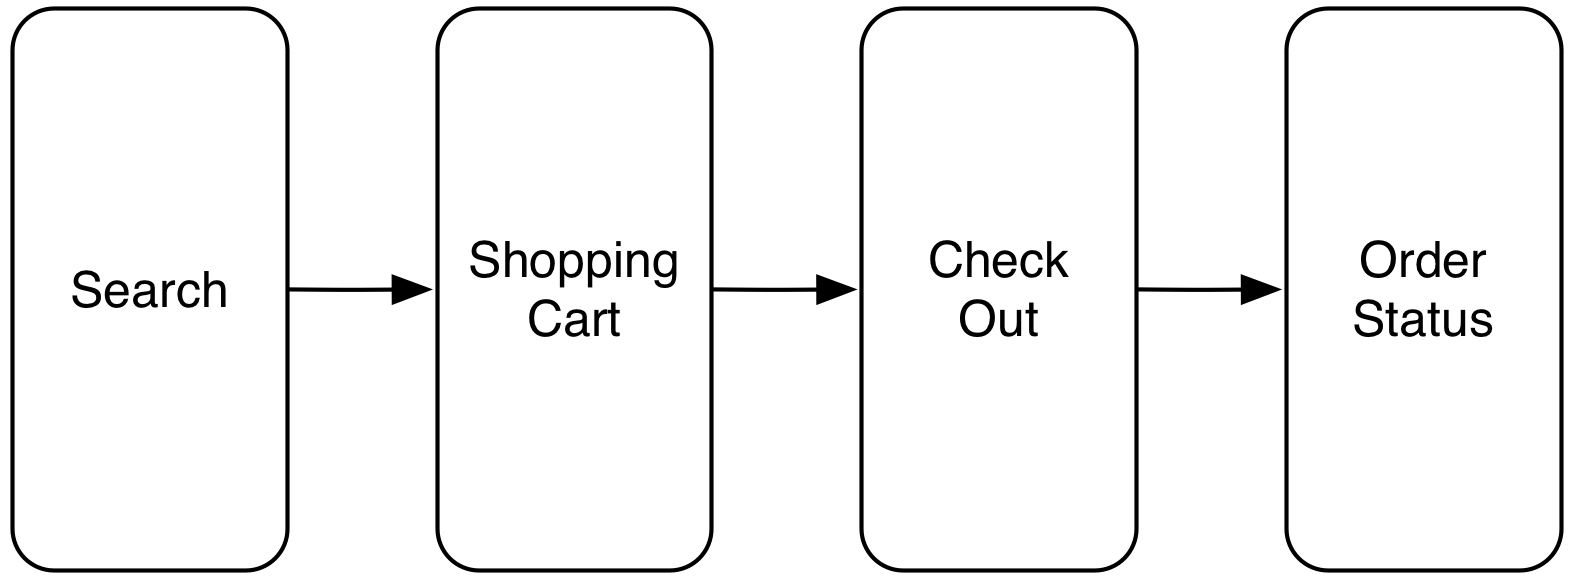
\includegraphics[scale=0.2]{pictures/Journey.png}
    \caption{Customer journey for an e-commerce system partitioned in various SCS \cite{scsWolf}}
    \label{fig:scsJourney}
\end{figure}

These fundamentals about micro services and self contained systems are quite important and will be mapped upon data warehouse architectures later on in chapter \ref{sec:finalArchitecture}.

\subsection{Integrating an Event-Based Bus into the Micro-Service Landscape}
\label{sec:eventBasedArchitecture}
Making use of an event-driven choreographed architecture is the opposite of using a centralised orechestrator and therefore provides a loose coupling. The ''EventBus allows publish-subscribe-style communication between components without requiring the components to explicitly register with one another (and thus be aware of each other).'' \cite{EventBusExplained} \newline
Another well known product which is often used in this context is Apache Kafka. It calls itself as ''distributed streaming platform'' having three key capabilities. First of all publishing and subscribing to streams, store streams as well as process streams.\cite{kafka}
Next up we are using this technology as an example in order to elaborate upon the challenges of this approach.\newline
\\
Bernd Rücker, who is Chief Technologist of Camunda, points those out quite well within an example. Therefore let's start by having a look upon the challenges:
\begin{itemize}
    \item How to change the flow of events?
    \item How to avoid losing sight of the flow?
    \item How to manage SLAs and resilience of the overall flow?
    \item How to avoid wired coupling?
\end{itemize}
\cite{eventDrivenMicroservices}\newline
\\
The illustration in figure \ref{fig:chalengesChoreographedMicroservices} shows how easily a loosely coupled choreographed system can result into dependencies. Bernd Rücker therefore choose the common customer on-boarding process to visualise it. The first illustration in figure \ref{fig:chalengesChoreographedMicroservices} shows the services and their flow of events. Furthermore he points out that by only adding one additional service to the overall system, such as a criminal check, will be followed by an adaption of at least two other services. This is shown in the second and alternatively third illustration.\cite{eventDrivenMicroservices}\newline
\begin{figure}[!htb]
    \centering
    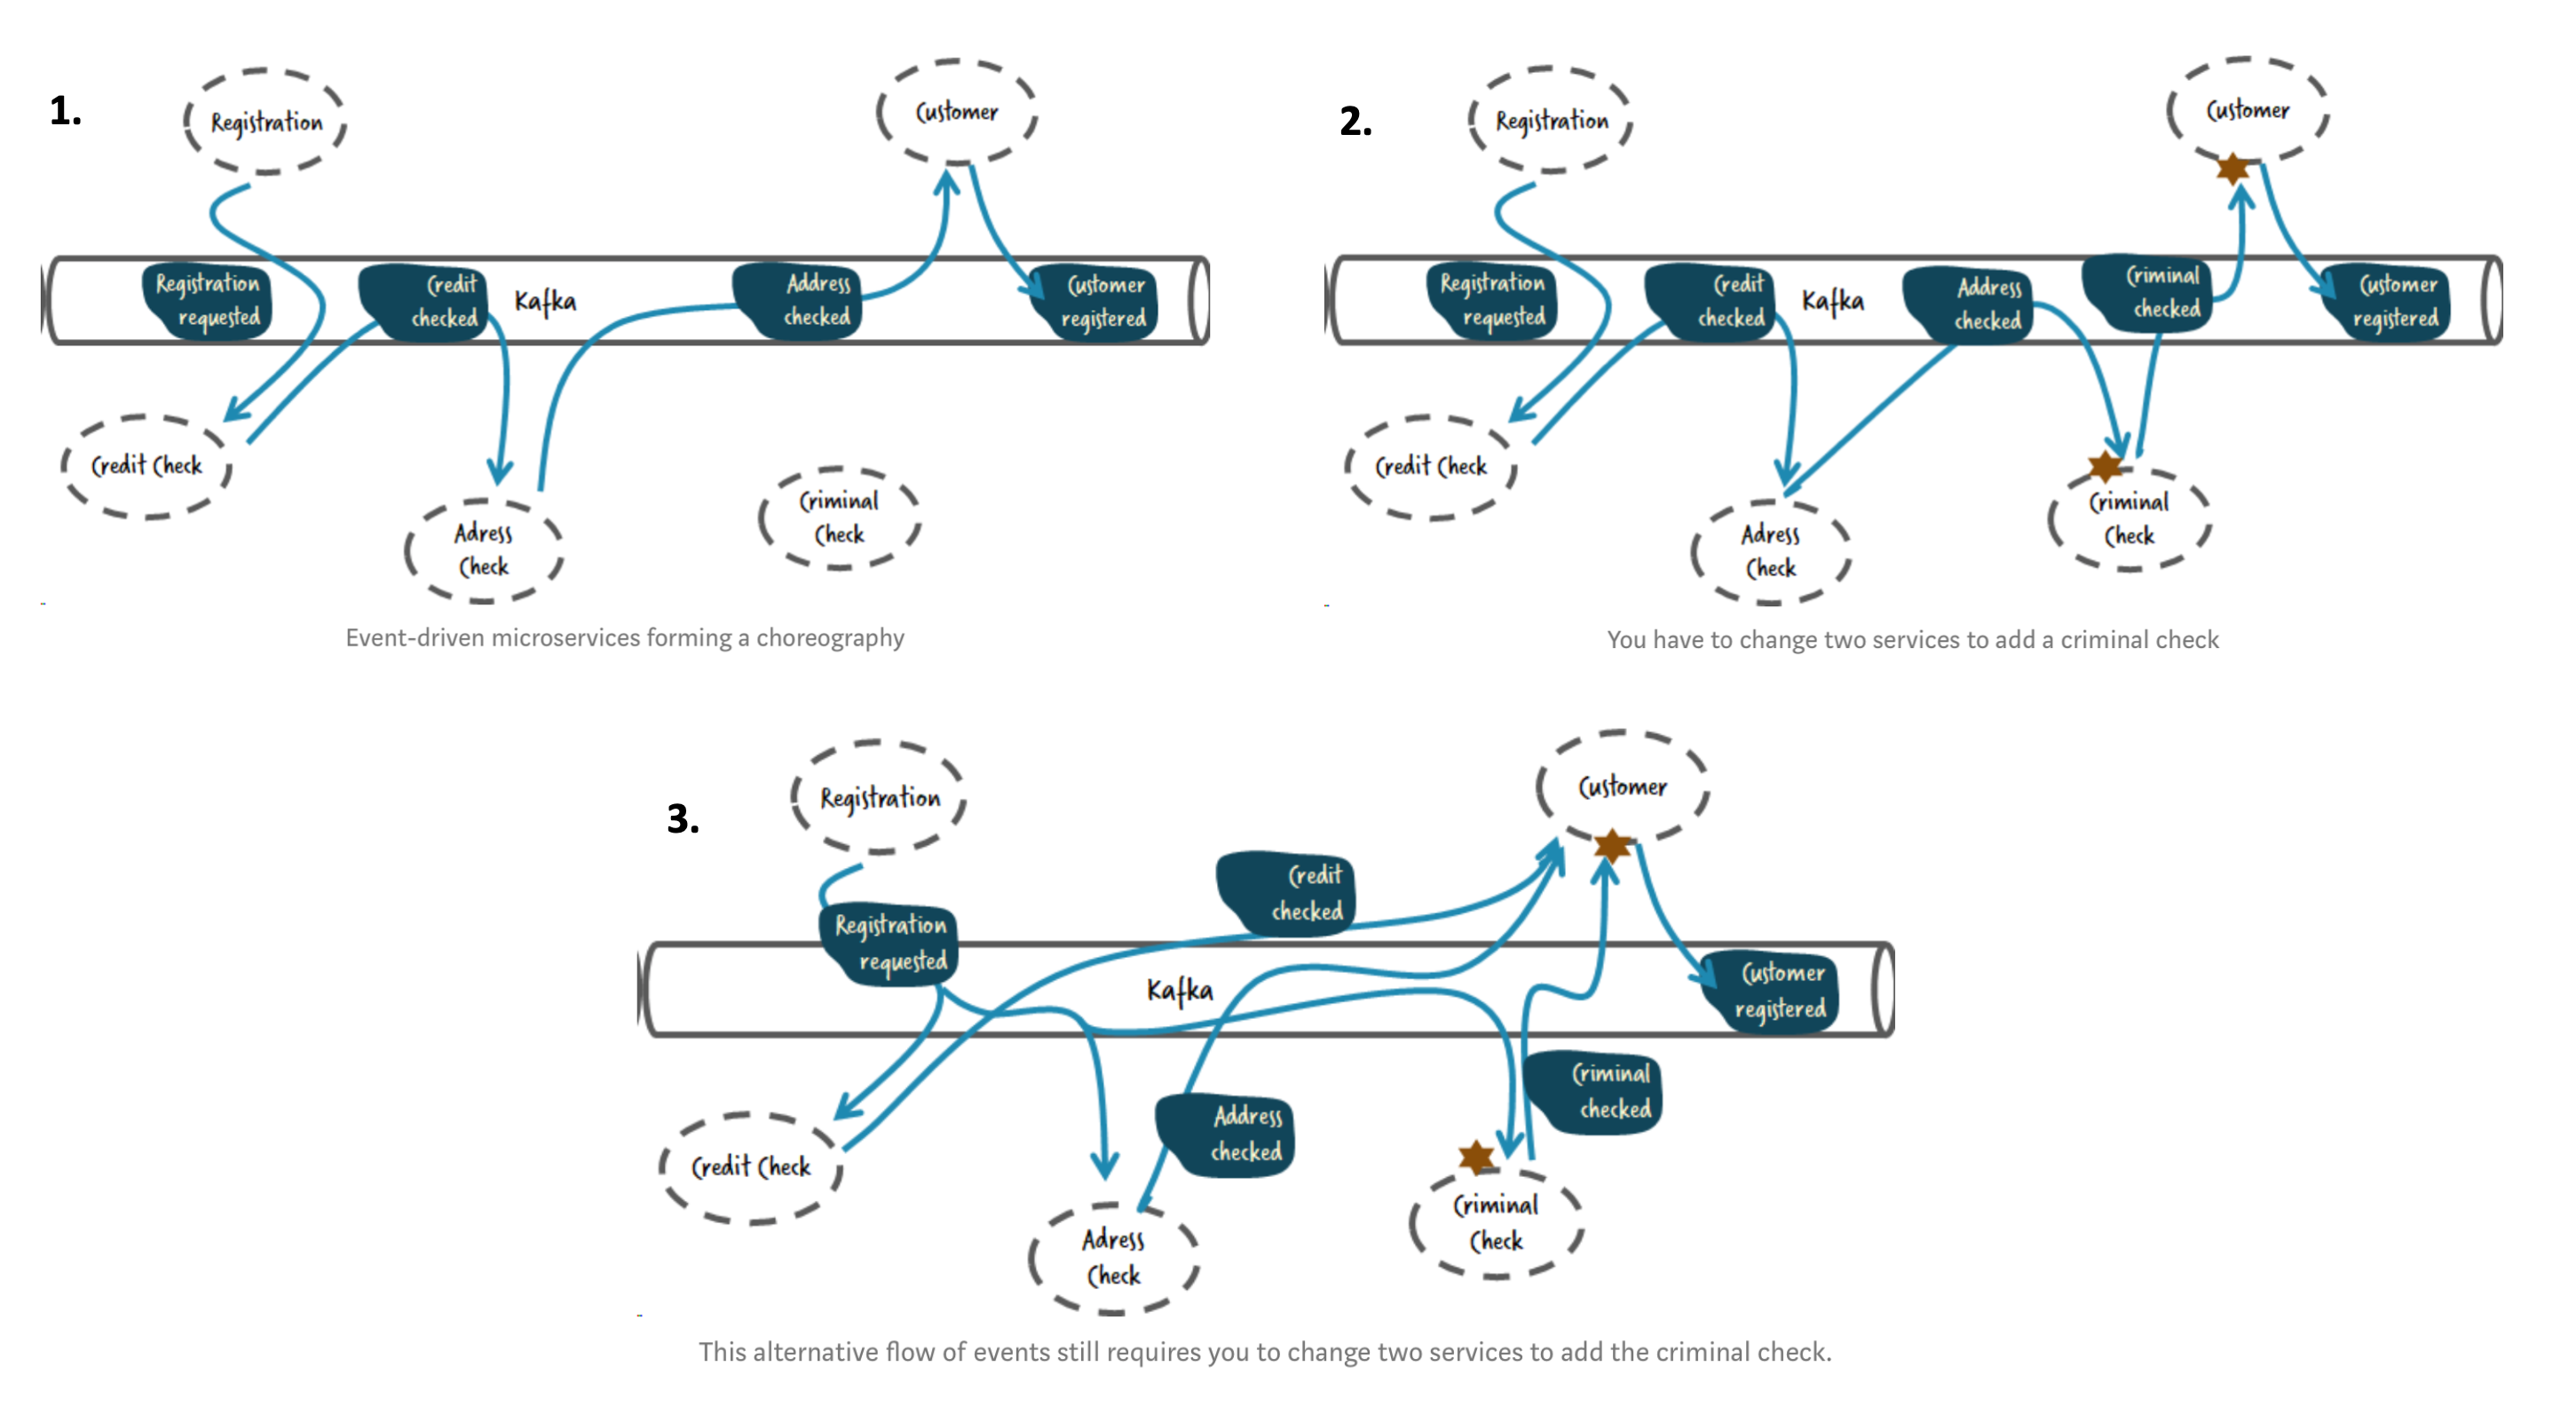
\includegraphics[scale=0.33]{pictures/FlowOfEvents.png}
    \caption{Challenges of choreographed microservices \cite{eventDrivenMicroservices}}
    \label{fig:chalengesChoreographedMicroservices}
\end{figure}

Summarised this problem combined with the ''emerging behaviour that will only be experienced during runtime''\cite{eventDrivenMicroservices} often lead into losing sight.\newline
Furthermore these faults can be seen as transition into the next chapter where the process driven architecture will be discussed. Nevertheless the similarities between microservices and self-contained-systems with regard to data warehouse systems can be pointed out quite well. The components which are known from the reference architecture in chapter \ref{sec:referenceArchitecture} figure \ref{fig:referenceArchitecture} can be sliced along the data warehousing process into distinct scs.\newline
The next section will now focus on how to orchestrate those properly without the challenges of an event-driven architecture. 